%
% teil1.tex -- Beispiel-File für das Paper
%
% (c) 2020 Prof Dr Andreas Müller, Hochschule Rapperswil
%
% !TEX root = ../../buch.tex
% !TEX encoding = UTF-8
%
\section{Unschärferelation
\label{sonogramm:section:teil1}}
\rhead{Unschärferelation}
Wie bereits in der Einleitung des Kapitels angedeutet sind die zusätzlichen
zeitlichen Informationen nicht gratis. 
Mit dem Aufteilen des ursprünglichen Signals in kurze Fenster bekommen wir eine
verbesserte zeitliche Auflösung, wir verlieren jedoch an Frequenzauflösung.
% In der Theorie ist die bestmögliche Frequenzauflösung 
% \begin{equation}
%     \Delta f = \frac{1}{T}
% \end{equation}
% wobei $T$ die zeitliche Länge der Fensterfunktion ist.
Zusätzlich werden durch das abrupte Abschneiden des Signals mit dem Rechteck-fenster
zusätzliche Frequenzen hinzugefügt. 
Diese Effekte hängen mit der Unschärferelation zusammen, welche in Abschnitt
\ref{buch:diskret:section:unschaerfe} genauer beschrieben ist.
%Dieser Effekt ist auch als "Frequency Leakage" bekannt.
In diesem Abschnitt werden wir diese Effekte genauer untersuchen.
\subsection{Auswirkung der Fensterfunktion}
Der Faltungssatz beschreibt 
\begin{align}
    f(t) * g(t)& \xrightarrow{\mathscr{F}} F(f)G(f),\\
    f(t) g(t)&\xrightarrow{\mathscr{F}}F(f) * G(f).
\end{align}
Das bedeutet, dass die Verwendung von Fensterfunktionen das Frequenzspektrum
des Signals mit dem Frequenzspektrum der Fensterfunktion gefaltet wird.
Die Fouriertransformation eines diskreten Rechteck-fensters ist 
\begin{equation}
    W_r(f) = \frac{\sin(2 \pi f  L_w / (2 f_s))}{\sin(2 \pi f / (2 f_s))} e^{-i 2 \pi f (L_w-1)/(2f_s)}
\end{equation}
mit $f_s$ als Abtastfrequenz.
% \begin{figure}
%     \centering
%     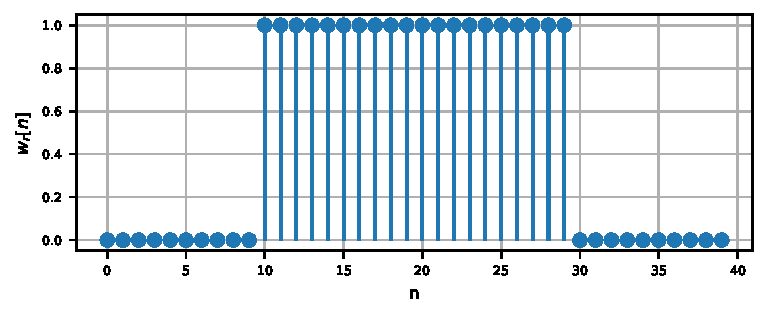
\includegraphics{papers/sonogramm/images/rect_time.pdf}
%     \caption{Rechtecksfenster mit $L_w = 20$.
%     \label{sonogramm:recttime}
%     }
% \end{figure}
\begin{figure}
    \centering
    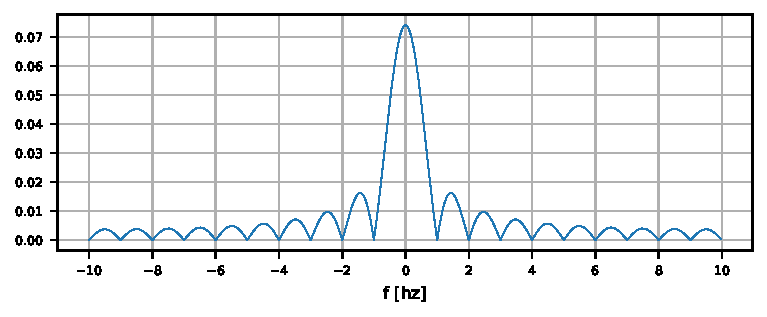
\includegraphics{papers/sonogramm/images/rect_freq.pdf}
    \caption{Frequenzspektrum eines ein Sekunden langes Rechteck-fensters mit Abtastfrequenz von 20 Hz. Die Nulldurchgänge sind jeweils bei ganzzahligen Vielfachen
    von $1/T$.
    \label{sonogramm:rectfreq}
    }
\end{figure}
In Abbildung \ref{sonogramm:rectfreq} sind zwei solche Frequenzspektren mit unterschiedlichen $L_w$ abgebildet.
Ideal wäre ein einzelner Peak bei 0, dafür müsste jedoch das Fenster eine Länge von $\infty$ haben.
Durch die Sprünge bei $n = 0$ und $n = L-1$ im Zeitbereich kommen zusätzliche Frequenzen dazu, der sogenannte
Leck-Effekt.
Diese unerwünschten Frequenzen werden durch die Faltung im Frequenzbereich zu den eigentlichen Frequenzen 
geschoben.
Abbildung \ref{sonogramm:leakageDemo} zeigt ein solches Spektrum eines Eintonsignals.
Man sieht wie die Leck-Frequenzen, vor allem beim kürzeren Signal,
sich über das ganze Spektrum verbreiten.
Schwächere Frequenzen können dabei im Spektrum von Leck-Frequenzen von dominanten Frequenzen
übertönt werden.
Die schwächeren Frequenzen sind dann entweder nicht erkennbar, oder es entsteht ein Peak 
bei einer falschen Frequenz. 
Abbildung \ref{sonogramm:leakageDemo2} zeigt das Spektrum von 
\begin{equation}
    f(t) = \sin(3.45\cdot 2\pi t) + 0.3  \cos(5.7\cdot  2\pi t)
\label{sonogramm:eq:sigLeck}
\end{equation}
mit 20 Hz über eine und fünf Sekunden gesampled.
Die Frequenz des Kosinus lässt sich mit einer Sekunde Messzeit nicht korrekt bestimmen, 
da die Leck-Frequenzen vom Sinus zu dominant sind.

Die Breite des Hauptpeaks limitiert die Frequenzauflösung.
Bei einem Rechteck-fenster ist dieser $2f_s/L_w$ Hz breit.
Sind zwei Frequenzen genügend nahe bei einander, überlappen sich die Hauptpeaks, und können
nicht mehr unterschieden werden. 
Zwei unterschiedliche Frequenzen können dadurch nur genau bestimmt werden wenn
\begin{equation}
    \Delta f \geq \frac{1}{T_w},
\end{equation}
was beim Rechteck-fenster gleich der halben Hauptpeak-Breite ist.
Die Annahme $\Delta f = 1/T_w$ ist jedoch mit Vorsicht zu gebrauchen, da $\Delta f$ je nach 
Phase der beiden Harmonischen grösser sein muss.
Abbildung \ref{sonogramm:freqdiffdemo} zeigt als Beispiel das Signal
\begin{equation}
    s(t) = \sin(2\pi 3.45 t ) + \sin (s\pi 4.45 t + \varphi)
    \label{sonogramm:eq:twoHarmPhi}
\end{equation}
mit $T_w = 1$ s, was eine Frequenzauflösung von maximal 1 Hz ergibt.
Je nach Phase des zweiten Sinus, können die Frequenzen unterschiedlich genau, oder sogar überhaupt nicht
bestimmt werden.
Wieso das so ist, lässt sich in der Zeit zeigen.
Werden zwei Sinuse mit einem kleinen $\Delta f$ addiert entsteht eine sogenannte Schwebung,
was im fall von \eqref{sonogramm:eq:twoHarmPhi}
\begin{equation}
    s(t) = \sin(2\pi 3.45 t ) + \sin (s\pi 4.45 t) = 2 \sin(2 \pi \frac{3.45 + 4.45}{2}t)
    cos(2 \pi  \frac{3.45 - 4.45}{2} t),
\label{sonogramm:eq:twoHarm}
\end{equation}
ergibt.
Abbildung \ref{sonogramm:twoHarmTime} zeigt \eqref{sonogramm:eq:twoHarm} über vier Sekunden.
Die Phase $\varphi$ bewirkt eine Verschiebung von \eqref{sonogramm:eq:twoHarm} in der Zeit, 
was bedeutet, dass abhängig von $\varphi$ ein anderer Abschnitt des Signales gefenstert wird.
Im Fall von $\varphi = \pi$ ist das gefensterte Segment genau zwischen zwei Nulldurchgänge
vom Kosinus.
Dies ist Äquivalent zu einem Sinus mit einer Frequenz von 3.95 Hz, welcher mit einem 
Sinus-fenster multipliziert wurde. 
Ein Sinus-fenster der Länge T ist ein 2T-periodischer Sinus, welcher nach T abgeschnitten wird.
Da damit die Phasensprünge nicht im gefensterten Bereich enthalten sind, 
gehen die Informationen über die eigentlichen addierten Sinuse verloren.
Ist $\varphi = 0$ ist der Phasensprung in der Mitte des Segmentes und damit optimal gelegen.

Man sollte daher mit der theoretischen Frequenzauflösung nicht ans Limit gehen, wenn man
zuverlässige Resultate erzielen möchte.

\begin{figure}
    \centering
    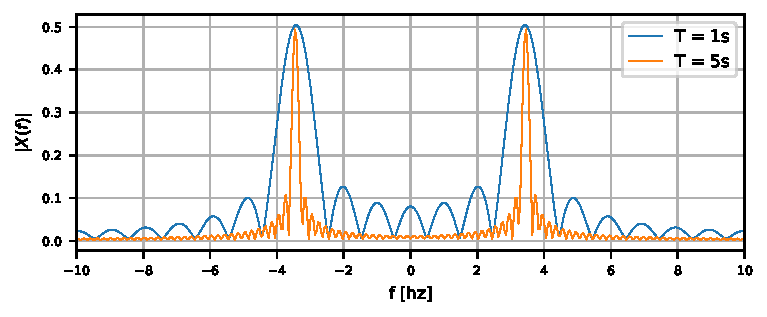
\includegraphics{papers/sonogramm/images/RectWinHarmEx.pdf}
    \caption{Frequenzspektrum Sinus mit Frequenz 3.45 Hz, welcher mit einem T langen 
    Rechteck-fenster zugeschnitten wurde.
    \label{sonogramm:leakageDemo}
    }
\end{figure}

\begin{figure}
    \centering
    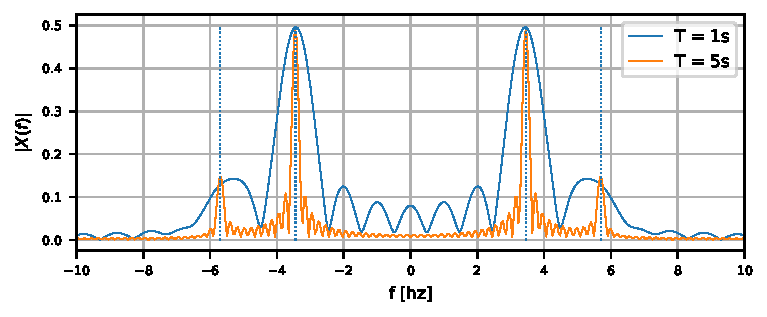
\includegraphics{papers/sonogramm/images/twohamrrect.pdf}
    \caption{Frequenzspektrum des Signals \eqref{sonogramm:eq:sigLeck}.
    Durch die Leck-Frequenzen kann bei einer kurzen Messzeit die Frequenz des Kosinus 
    nicht richtig bestimmt werden.
    \label{sonogramm:leakageDemo2}
    }
\end{figure}

\begin{figure}
    \centering
    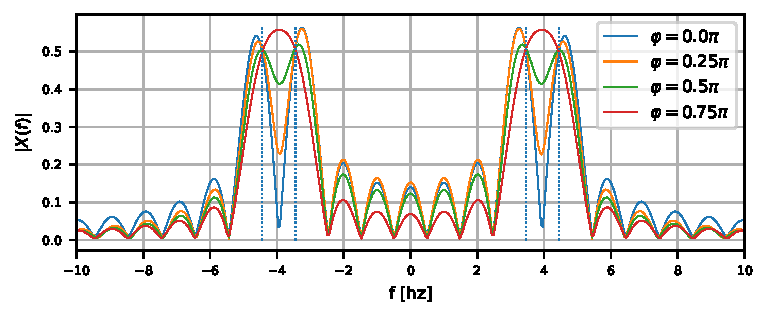
\includegraphics{papers/sonogramm/images/twoharmphasediff.pdf}
    \caption{Frequenzspektrum eines Zweitonsignals mit $\Delta f = 1$ Hz.
    Je nach Phasenunterschied der beiden Sinuse, lassen sich die Frequenzen unterschiedlich
    genau bestimmen.
    \label{sonogramm:freqdiffdemo}
    }
\end{figure}

\begin{figure}
    \centering
    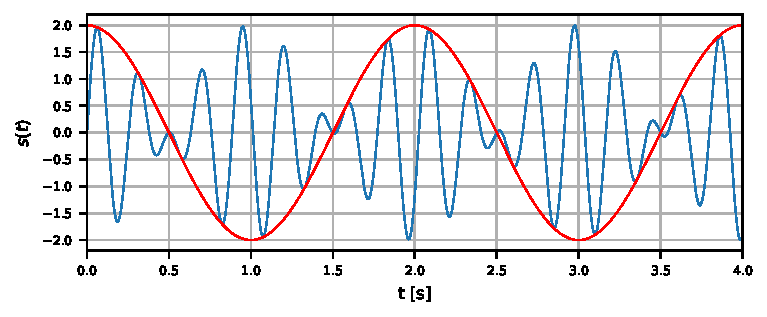
\includegraphics{papers/sonogramm/images/twoharmTime.pdf}
    \caption{Funktion in \eqref{sonogramm:eq:twoHarm} über 4 Sekunden in blau, und der resultierende
    umhüllende Kosinus in rot.
    Bei den Nulldurchgängen hat der multiplizierte Sinus der Frequenz 3.95 Hz Phasensprünge.
    \label{sonogramm:twoHarmTime}
    }
\end{figure}

\subsection{Andere Fensterfunktionen}
Bis jetzt haben wir uns auf das Rechteck-fenster beschränkt.
Dieses eignet sich zwar gut um die theoretischen Grundlagen zu zeigen,
es ist aber nicht immer das beste.

Wie im vorherigen Abschnitt aufgezeigt, sind die Frequenzauflösung und 
Leck-Frequenzen abhängig von der Fensterfunktion.
Durch die abrupten Sprünge im Rechteck-fenster sind die Leck-Frequenzen 
über ein weites Frequenzband sehr prominent.
Um dies zu verbessern wäre os besser eine Fensterfunktion zu haben,
welche bei $n = 0$ einen Wert nahe bei 0 hat,
bis zur Mitte des Fensters auf 1 steigt um dann bis $n = L_w -1$ wieder Richtung 0 zu gehen. 


Eine bekannte Funktion, welche solche Eigenschaften aufweist ist die gausssche Glockenkurve
\begin{equation}
    f(t) = e^{-\frac{t^2}{\alpha}}
\end{equation}
wobei $\alpha$ ein frei wählbarer Parameter ist, welcher die Breite der Glocke 
bestimmt.
Damit wir sehen, wie sich ein Gauss-fenster auf das Signal auswirkt, brauchen wir
die Fouriertransformation einer gaussschen Glocke.
Diese berechnet sich mit 
\begin{align}
    W_g(f) &= \int_{-\infty}^{\infty} e^{-\frac{t^2}{\alpha}} e^{- 2 \pi i f t}\, dt\\
    &= \int_{-\infty}^{\infty} e^{-\frac{t^2}{\alpha}} \cos(2 \pi f t)\, dx -
    i \int_{-\infty}^{\infty} e^{-\frac{t^2}{\alpha}} \sin(2 \pi f t)\, dx .
\end{align}
Das zweite Integral ist 0, da wir eine ungerade Funktion von $-\infty$ bis $\infty$ integrieren.
Die Lösung des ersten Integrals lässt sich mit der Integral Tabelle in \cite{sonogramm:bronstein} finden und ist mit
\begin{equation}
    W_g(f) = \int_{-\infty}^{\infty} e^{-\frac{t^2}{\alpha}} \cos(2 \pi f t)\, dt =
    \frac{\sqrt[2]{\alpha \pi}}{2} e^{-\alpha \pi^2 f^2}
\end{equation}
wieder eine Gausssche Glocke, bei welcher der Parameter $\alpha$ invertiert vorkommt.
Das bedeutet, dass eine in der Zeit schmale Gausssche Glocke ein breites Frequenzspektrum hat und umgekehrt eine
breite Gausssche Glocke in der Zeit ein schmales Frequenzspektrum hat.
Das Deckt sich mit unseren Beobachtung bezüglich dem Zusammenhang der 
Frequenzauflösung und der Länge eines Fensters.

In Abbildung \ref{sonogramm:gausstime} sind zwei Gauss-fenster mit unterschiedlichen 
$\alpha$ abgebildet.
Da das Fenster einer STFT eine endliche Länge hat, müssen wir die Gaussschen Glocken 
mit einem Rechteck-fenster zuschneiden. 
Somit wird es wieder Leck-Frequenzen geben, die aber je nach $\alpha$ viel kleiner sind
als beim Rechteck-fenster, wie in Abbildung \ref{sonogramm:gaussfreq} zu sehen ist.
Ausserdem sehen wir, dass die Hauptpeaks der Gauss-fenster breiter sind als der 
Hauptpeak des Rechteck-fensters.
Allgemein gilt das Rechteck-fenster als optimal bezüglich der Frequenzauflösung.
Wir bezahlen also die Minimierung der Leck-Frequenzen mit einer kleineren Frequenzauflösung. 
Mit einem passend gewählten $\alpha$ kann man somit die Fensterfunktion auf eine spezifische
Anwendung optimieren.

\begin{figure}
    \centering
    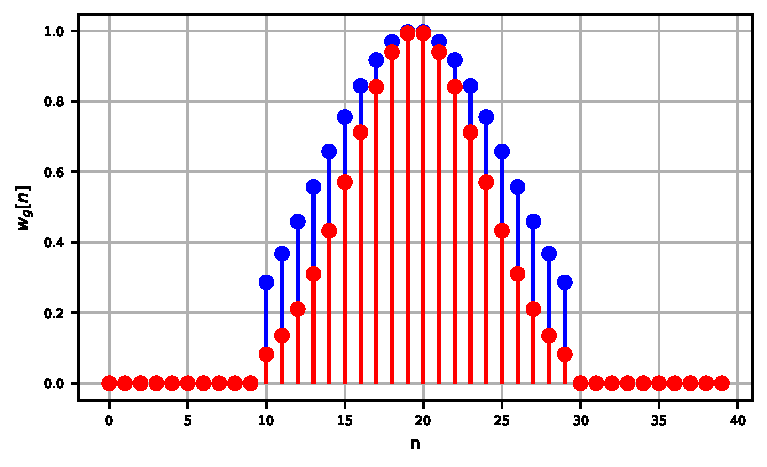
\includegraphics{papers/sonogramm/images/gauss_time.pdf}
    \caption{Gauss Fenster mit $L_w = 20$ mit unterschiedlichen $\alpha$.
    \label{sonogramm:gausstime}
    }
\end{figure}

\begin{figure}
    \centering
    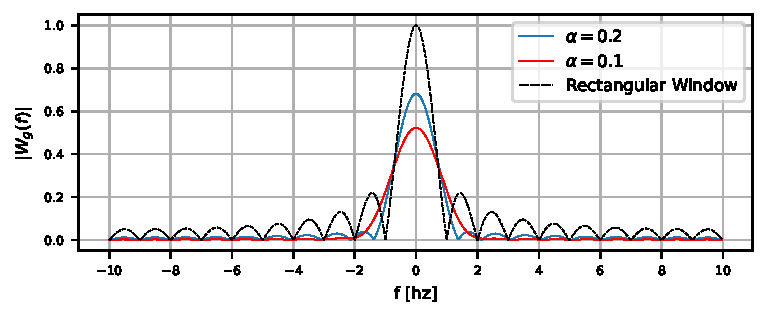
\includegraphics{papers/sonogramm/images/gauss_freq.pdf}
    \caption{Frequenzspektrum der Gauss-fenster von Abbildung \ref{sonogramm:gausstime}
    mit einer Abtastfrequenz von 20 Hz. Zum Vergleich ist in schwarz das Spektrum eines Rechteck-fenster 
    von der selben Länge.
    von $1/T$.
    \label{sonogramm:gaussfreq}
    }
\end{figure}

Nehmen wir das Signal \eqref{sonogramm:eq:sigLeck} und wenden statt dem Rechteck-fenster
ein Gauss-fenster an, resultiert das Frequenzspektrum in Abbildung \ref{sonogramm:twoHarmGauss}.
Der Kosinus lässt sich somit beim kürzeren Signal genauer bestimmen.
$\alpha$ musste dabei sorgfältig gewählt werden, da bei einem zu kleinen $\alpha$ die 
Frequenzauflösung zu klein gewesen wäre, und bei einem zu grossen $\alpha$ die Leck-Frequenzen
noch immer dominiert hätten.

\begin{figure}
    \centering
    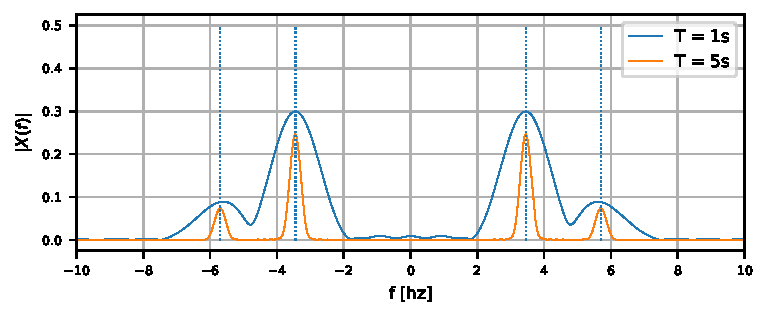
\includegraphics{papers/sonogramm/images/twoHarmGauss.pdf}
    \caption{Frequenzspektrum des Signals \eqref{sonogramm:eq:sigLeck} mit
    einem Gauss-fenster. Das Spektrum ist bei den Frequenzen, welche nicht im Signal vorkommen
    nun beinahe bei 0.
    \label{sonogramm:twoHarmGauss}
    }
\end{figure}

Das Gauss-fenster ist eine von vielen Fensterfunktionen. 
Eine beste Fensterfunktion gibt es nicht, denn jede hat ihre Vor- und Nachteile, welche
je nach Anwendung anders gewichtet werden.
Für interessierte Leser bietet \cite{sonogramm:wikiWin} eine 
gute Übersicht anderer Fensterfunktionen.

